\documentclass[aspectratio=169]{beamer}

\usepackage[utf8]{inputenc}
%\usepackage{latexsym}
\usepackage{graphicx}
\usepackage{mathptmx}
\usepackage{amsmath}
%\usepackage{amsfonts}
\usepackage{amssymb}
\usepackage{amsbsy}
\usepackage{amsthm}
\usepackage{algorithmic}

% Get checkmark logo
\usepackage{pifont}
\newcommand{\cmark}{\ding{51}}
\newcommand{\xmark}{\ding{55}}
% Get \lee and \gee commands
\newcommand{\lee}{\leqq}
\newcommand{\gee}{\geqq}

% Strikouts
\usepackage[normalem]{ulem}

% Restore Mathcal
\let\saveboldmath\boldmath
\usepackage{mathptmx}
\let\boldmath\saveboldmath
\usepackage{bm}
\DeclareSymbolFont{cmsymbols}{OMS}{cmsy}{m}{n}
\SetSymbolFont{cmsymbols}{bold}{OMS}{cmsy}{b}{n}
\DeclareSymbolFontAlphabet{\mathcal}{cmsymbols}

\usepackage[english]{babel}
\usepackage[utf8]{inputenc}

% AMSLaTeX packages
\usepackage{amsthm}
\usepackage{amsmath}
\usepackage{amsfonts}
\usepackage[algoruled]{algorithm2e}

\usetheme{default}
\useoutertheme{default}
% we want to use images
\usepackage{graphicx}
\usepackage{movie15}
\usepackage{hyperref}

% table relates packages
\usepackage{booktabs}
\usepackage{multirow}
% pick a font
\usepackage{palatino}           
% \usepackage{times}
\usepackage{tikz}
\usetikzlibrary[positioning,arrows,decorations.pathmorphing,backgrounds,fit,calc]
% \AtBeginSection[]  % "Beamer, do the following at the start of every section"
% {
%   \begin{frame}<beamer> 
%     \frametitle{Outline} % make a frame titled "Outline"
%     \tableofcontents[currentsection]  % show TOC and highlight current section
%   \end{frame}                    
% }

% \AtBeginSubsection[]
% {
%   \begin{frame}
%     \frametitle{Outline}
%     \tableofcontents[currentsection,currentsubsection]
%   \end{frame}
% }

\AtBeginSection[]
{
   \begin{frame}
       \frametitle{Outline}
       \tableofcontents[currentsection]
   \end{frame}
}

\newcommand{\ebox}[1][1em]{\framebox[#1]{\phantom{M}}}

\setlength\arraycolsep{1.4pt}% some length

%gets rid of navigation symbols
\setbeamertemplate{navigation symbols}{}

%gets rid of bottom navigation bars
\setbeamertemplate{footline}[page number]{}
\setbeamertemplate{headline}{}


\usebackgroundtemplate{\includegraphics[width=\paperwidth]{../templates/NormalANLBlue}}
% Title Information
\title{The curse of dimensionality}
\author{Tyler Chang}
\date{CAA\&CM Argonne Student Visit\\
Sep 28, 2023}
\institute{Argonne National Laboratory}

\begin{document}

\setbeamertemplate{footline}{}
{
\usebackgroundtemplate{\includegraphics[width=\paperwidth]{../templates/TitleANLBlue}}
\frame{\titlepage}
}

\setbeamertemplate{footline}[page number]{}

%% FRAME: overview
%\begin{frame}
%  \frametitle{Outlines}
%  \tableofcontents
%\end{frame}

\section{Everything is a function}

\begin{frame}\frametitle{Everything is a function}

\pause
{\large
$$
f(x_1, x_2, x_3, \ldots, x_n) \rightarrow y
$$
}

\pause
\bigskip

\begin{tabular}{c}
\includegraphics[width=0.1\textwidth]{../img/delaunay_new/mnist_data_0.png}
\end{tabular}
{\huge $\quad \xrightarrow{ f } \quad 0$}
$\qquad\qquad\quad$
\pause
\begin{tabular}{c}
{\large ``The dog jumped}\\
{\large over the ...''}
\end{tabular}
{\huge $\quad \xrightarrow{ f }$}
{\large $\quad$ ``fence''}
\end{frame}

\begin{frame}\frametitle{Everything is a function}

{\large
$$
f(x_1, x_2, x_3, \ldots, x_n) \rightarrow y
$$
}

\pause
\bigskip

\begin{columns}
\begin{column}{0.5\textwidth}
\begin{center}
\includegraphics[height=5em]{../img/probs/cfr-nmr-setup.jpg}\\
{\small
Molecular discovery for better battery electrolytes
(photo from the Argonne MERF).\\
}
\end{center}
\end{column}

\pause

\begin{column}{0.5\textwidth}
\begin{center}
\includegraphics[height=5em]{../img/probs/nasa-f15.png}\\
{\small
Nonparametric aircraft geometry (photo from NASA Langley).\\
}
\end{center}
\end{column}
\end{columns}

\pause

\begin{center}
\includegraphics[height=4em]{../img/moo_new/accelerator_design.png}\\
{\small
Particle accelerator designs (photo from simulation run on HPCs at Argonne).\\
}
\end{center}

\end{frame}

\section{The fundamental ML problem (multidimensional inference)}

\begin{frame}\frametitle{The fundamental machine learning problem}

\begin{columns}
\begin{column}{0.5\textwidth}

\onslide<2>{
\begin{center}
\includegraphics[width=\textwidth]{../img/delaunay_new/inference_1d_pt1.eps}
\end{center}
}

\onslide<3>{
\begin{center}
\vskip -14.5em
\includegraphics[width=\textwidth]{../img/delaunay_new/inference_1d_pt2.eps}
\end{center}
}

\onslide<4>{
\begin{center}
\vskip -14.5em
\includegraphics[width=\textwidth]{../img/delaunay_new/inference_1d_pt3.eps}
\end{center}
}

\onslide<5>{
\begin{center}
\vskip -14.5em
\includegraphics[width=\textwidth]{../img/delaunay_new/inference_1d_pt4.eps}
\end{center}
}

\onslide<6>{
\begin{center}
\vskip -14.5em
\includegraphics[width=\textwidth]{../img/delaunay_new/inference_1d_pt5.eps}
\end{center}
}

\end{column}
\begin{column}{0.5\textwidth}
\begin{itemize}
\onslide<2->{\item Want to predict unknown $f(x)$ for observation $x$}
\onslide<3->{\item {\bf ML}: {\sl Learn} approximation ${\hat f} \sim f$ based on {\sl training data} ${\cal X}$}
\onslide<3->{\item {\bf NA}: fit an interpolant (piecewise-linear) to $f$ on ${\cal X}$}
\onslide<4->{\item Both cases: more data $\Rightarrow$ better ${\hat f}$}
\onslide<5->{\item Real data not perfectly balanced  $\Rightarrow$ ${\hat f} \rightarrow f$ non-uniformly}
\onslide<6->{\item If we have enough data, it doesn't matter}
\end{itemize}
\end{column}
\end{columns}

\end{frame}

\section{The curse of dimensionality}

\begin{frame}
\frametitle{The curse of dimensionality}

\begin{columns}
\begin{column}{0.5\textwidth}
\begin{center}
\includegraphics[width=0.8\textwidth]{../img/delaunay_new/inference_2d_pt1.eps}\\
10 training points in 1D
\end{center}
\end{column}

\begin{column}{0.5\textwidth}
\begin{center}
\includegraphics[width=0.95\textwidth]{../img/delaunay_new/inference_2d_pt2.eps}\\
10 training points in 2D
\end{center}
\end{column}
\end{columns}
\end{frame}

\subsection{Not enough data to make accurate predictions}

\begin{frame}
\frametitle{The curse of \sout{dimensionality} no data}

\begin{columns}
\begin{column}{0.5\textwidth}
\begin{center}
\includegraphics[width=0.8\textwidth]{../img/delaunay_new/inference_2d_pt3.eps}\\
Need data in all quadrants?
\end{center}
\end{column}

\begin{column}{0.5\textwidth}
\pause
\begin{itemize}
\item Inference in 2D : $2^2 = 4$
\item Inference in 10D : $2^{10} \approx 1000$
\item Inference in 100D : $2^{100} \approx 10^{30}$ (orders of magnitude bigger than exascale)
\item Many ML problems : inference in 1000+ dimensions
\end{itemize}
\end{column}
\end{columns}
\end{frame}

\subsection{Too much data for many ``classical'' methods}

\begin{frame}\frametitle{The curse of \sout{dimensionality} too much data}

Classical methods to ``connect the dots'' in high-dimensions
(from applied math literature) rely on meshing:

\begin{columns}
\begin{column}{0.5\textwidth}
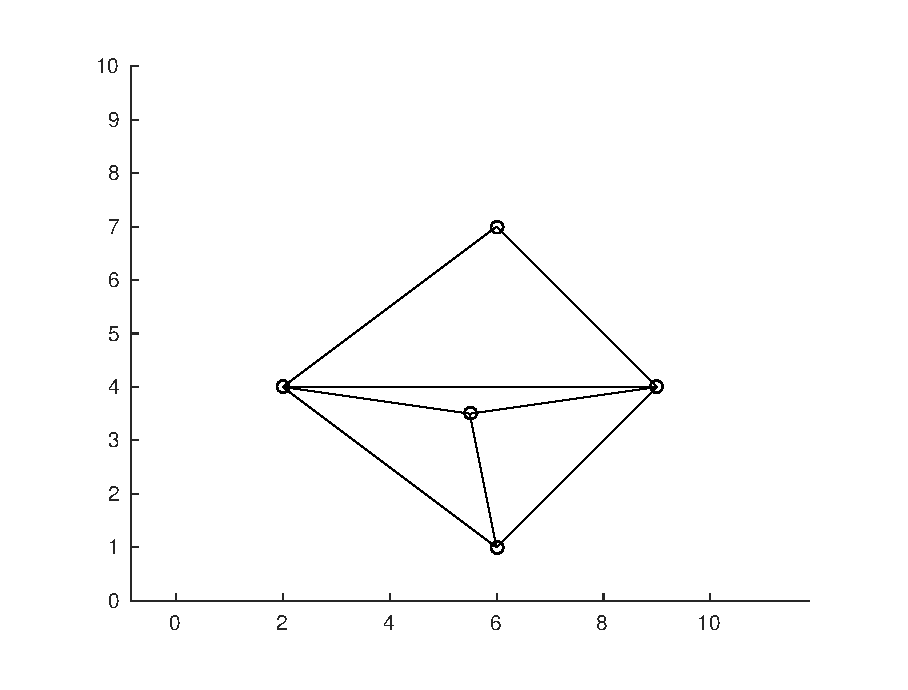
\includegraphics[width=0.9\textwidth]{../img/delaunay_old/triangleplane.eps}
\end{column}
\begin{column}{0.5\textwidth}
\begin{itemize}
\pause \item A mesh of $n$ points in $\mathbb{R}^d$ can have up to
${\cal O}(n^{d/2})$ elements
\pause \item Takes {\bf at least} ${\cal O}(n^{d/2})$ time to compute
\pause \item Requires {\bf at least} ${\cal O}(n^{d/2})$ storage
\pause \item {\bf Impossible for large data sets}
\end{itemize}
\end{column}
\end{columns}
\end{frame}

\section{Data from some existing methods}
\begin{frame}\frametitle{Results for some methods}
\begin{center}
\includegraphics[width=0.9\textwidth]{../img/delaunay_new/wind_results_tyler.png}
\end{center}
\end{frame}

\begin{frame}\frametitle{Results for some methods}
\begin{center}
\includegraphics[width=0.9\textwidth]{../img/delaunay_new/wind_results_you.png}
\end{center}
\end{frame}

\begin{frame}
  \frametitle{Questions}
  \tableofcontents
  \bigskip
\end{frame}

%%% Bonus slides %%%

\begin{frame}\frametitle{Some courses to take}
\begin{columns}
\begin{column}{0.5\textwidth}
Math:
\begin{itemize}
\item Advanced linear algebra
\item Numerical analysis
\item Functional analysis
\end{itemize}
\end{column}
\begin{column}{0.5\textwidth}
CS:
\begin{itemize}
\item Data structures \& algorithms
\item Parallel computing
\item Data analysis and/or Machine learning
\end{itemize}
\end{column}
\end{columns}
\end{frame}

\end{document}
